%%%%%%%%%%%%%%%%%%%%%%%%%%%%%%%%%%%%%%%%%%%%%%%%%%%%%%%%%%%%%%%%%%%
%                                                                 %
%                            APPENDICES                           %
%                                                                 %
%%%%%%%%%%%%%%%%%%%%%%%%%%%%%%%%%%%%%%%%%%%%%%%%%%%%%%%%%%%%%%%%%%%
 
\appendix    % This command is used only once!
%\addcontentsline{toc}{chapter}{APPENDICES}             %toc entry  or:
\addtocontents{toc}{\parindent0pt\vskip12pt APPENDICES} %toc entry, no page #

\chapter{Name Server Options and System Properties}\label{nameserverop}
  \section{Name Server Options}
    The name server can be run with several arguments. Running the name server 
    with the command {\tt -h} provides all the possible options.\\
    {\tt java wwc.naming.NamingServer -h
	  \begin{description}
	  \item {usage:
		\begin{description}
		\item java ...WWCNamingServer
		\item java ...WWCNamingServer -h
		\item java ...WWCNamingServer -v
		\item java ...WWCNamingServer -p portNumber
		\end{description}
	  }
	  \item {options:
		\begin{description}
		\item -h: Print this message.
		\item -v: Print version number.
		\item -p portNumber: Set the listening port to portNumber. Default port number is $3030$.
		\end{description}                  
	  }
	  \end{description} 
	}

  \section{System Properties}
	
	{SALSA programs can be executed with a set of system properties:
	  {\tt
		\begin{description}
		\item -Dport=<port number>: To specify the port number that the 
                 automatically started theater will listen to. Otherwise, a random port number is used.
		\item -Didentifier=<id>: To specify the relative locator of the bootstrapping actor's UAL.
		\item -Duan = <uan>: To specify the UAN of the bootstrapping actor.
		\item -Dual= <ual>: To specify the UAL of the bootstrapping actor.
		\item -Dnogc: The local garbage collector will not be triggered
		\item -Dgcverbose: To show the behavior of local GC
		\item -Dnodie: Making a dynamically created theater alive
		\end{description}
	  }
	}
    {
		Here comes the example: \begin{description}
		\item {\tt java -Dport = 5050 -Didentifier = actor/hello HelloWorld}
		\end{description}
	}
    {
		A theater is started at the current host (e.g. {\tt europa.wcl.cs.rpi.edu}).
		The dynamically created theater listens on port $5050$, and 
		the {\tt HelloWorld} actor has the UAL:  \begin{description}
		\item {\tt rmsp://europa.wcl.cs.rpi.edu:5050/actor/hello}
		\end{description}
	}

\chapter{Debugging Tips}\label{DebuggingTips} {
\begin{itemize}
\item Make sure you really understand the actor model, its message passing semantics, and
the concurrency coordination abstractions built in SALSA. 

\item Message passing and remote procedure
calls are totally different. A named token variable does not have the 
result immediately. It has the result only after the message gets 
executed.

\item Objects in messages have pass-by-value semantics. This means that object arguments are
cloned and then sent. A latter modification on these object arguments does not change
the objects which were originally sent. 

\item Since the SALSA compiler does not support type checking in this version,
you may need to go through the Java source code. The code related to your
program is on the bottom of the generated Java source code. Do not try 
to modify other parts irrelevant to your SALSA source code.

\item Please note that a typo in a message sending statement does not
generate Java or SALSA compile-time errors. You have to be very careful with that.
A run-time error will be generated instead.

\item Most people confuse {\tt self} with {\tt this}. {\tt this} means "this actor", 
while {\tt self} "the actor reference" pointing to itself. {\tt self} can only be used 
as a target of messages, or an argument to be passed around. {\tt this} can be used for 
object method invocation. To send your references to other actors,
use  {\tt self}. Using {\tt this} is wrong.
\end{itemize}
}

\chapter{Learning SALSA by Example Code}\label{LearningSALSAEx}{
One can download the SALSA source code at
\begin{description}
\item {\tt http://wcl.cs.rpi.edu/salsa/}, 
\end{description}
which includes several good examples.

\section{Package {\tt examples}}
Package {\tt examples} are useful for learning SALSA. Examples consist of:
\begin{itemize}
\item {\tt examples.addressbook}: The address book example shown in 
Section~\ref{How SALSA Supports the Worldwide Computing Model}.
\item {\tt  examples.cell}: It implements a cell actor that has two message handlers: 
{\tt set} to set the value, and {\tt get} to get the value of the cell.  
Both versions of distributed and single host examples are provide.
\item {\tt examples.chat}: Two {\tt Speaker} actors run as services and start 
a chat session which is triggered by the {\tt Chat} actor.
\item {\tt examples.fibonacci}: The recursive {\tt fibonacci} application.
\item {\tt examples.Heat}: A simple simulation of heat flow. Both distributed and 
single host versions are provided.
\item {\tt examples.helloworld}: The {\tt HelloWorld} example.
\item {\tt examples.messenger}: An example showing message delivery.
\item {\tt examples.migration}: An example to show how to migrate an actor.
\item {\tt examples.multicast}: A group of examples showing how to implement several multicast protocols.
\item {\tt examples.nqueens}: A program that tries to solve the 
N-Queens problem.
\item {\tt examples.numbers}: Examples of actor inheritance and concurrency
coordination.
\item {\tt examples.ping}: An example showing the echo server and the ping client.
\item {\tt examples.ticker}: A ticker example: a non-terminating actor
\item {\tt examples.trap}: This numerical application approximates the integral of a function over 
an interval [a, b] by using the trapezoidal approximation.
\end{itemize}

\section{Package {\tt tests}}
Package {\tt  tests} is used for testing SALSA, including language
and run-time environment tests.
\begin{itemize}
\item {\tt  tests.language}: Tests for SALSA language constructs.
\item {\tt  tests.language.babyfood}: Tests for inheritance.
\item {\tt  tests.localgc}: Correctness tests for local actor garbage collection.
\item {\tt  tests.distributed}: Correctness tests for distributed actor garbage collection.
\end{itemize}
}

\chapter{Visualization of SALSA Applications with OverView}\label{OverViewVisualization}
\section{Introduction}
OverView is a toolkit for visualization of distributed systems, and is designed to be generic (that is, able to be applied to many different distributed systems), scalable (that is, to scale up to very large distributed systems), and dynamic (that is, functioning as well online as it does offline). OverView is written in Java and is designed to work with any arbitrary Java system via a custom unintrusive profiling mechanism and a simple declarative language (called the Entity Specification Language) which describes how to map Java method invocations into a high-level description of visualization events. Figure \ref{heatExample} shows how OverView visualizes an actor creation event.

\begin{figure}
\begin{tabular}{lll}
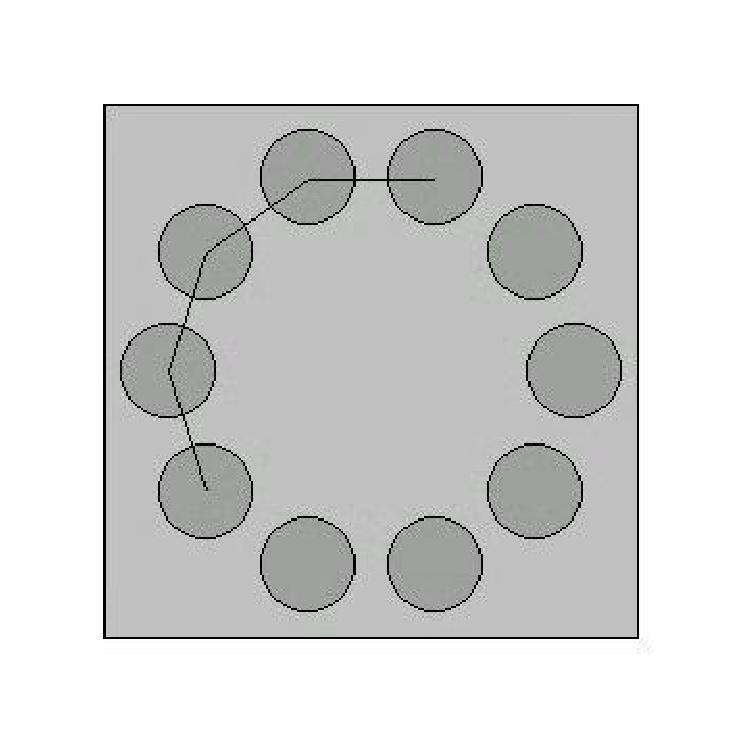
\includegraphics[angle=0,scale=0.3]{heatavi1.eps} & 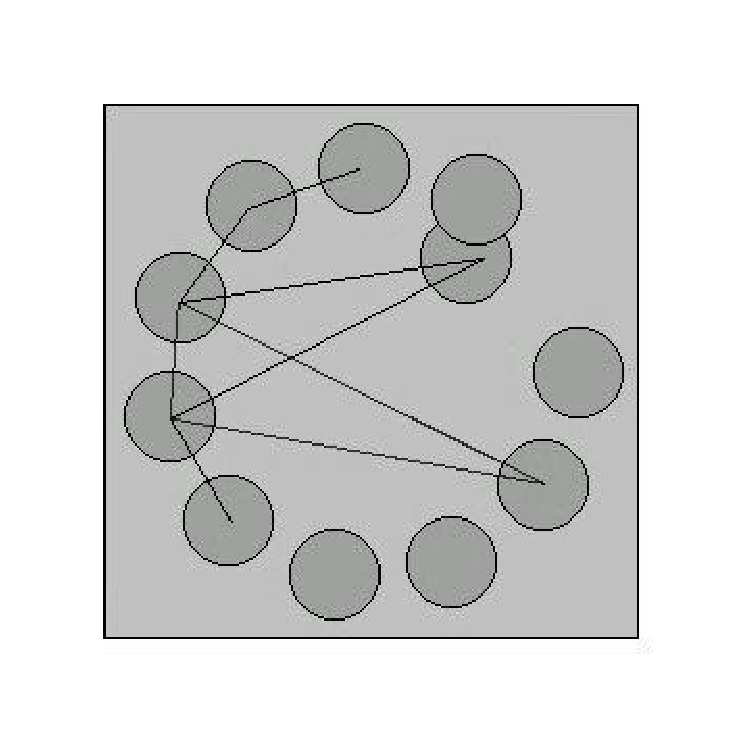
\includegraphics[angle=0,scale=0.3]{heatavi2.eps} &
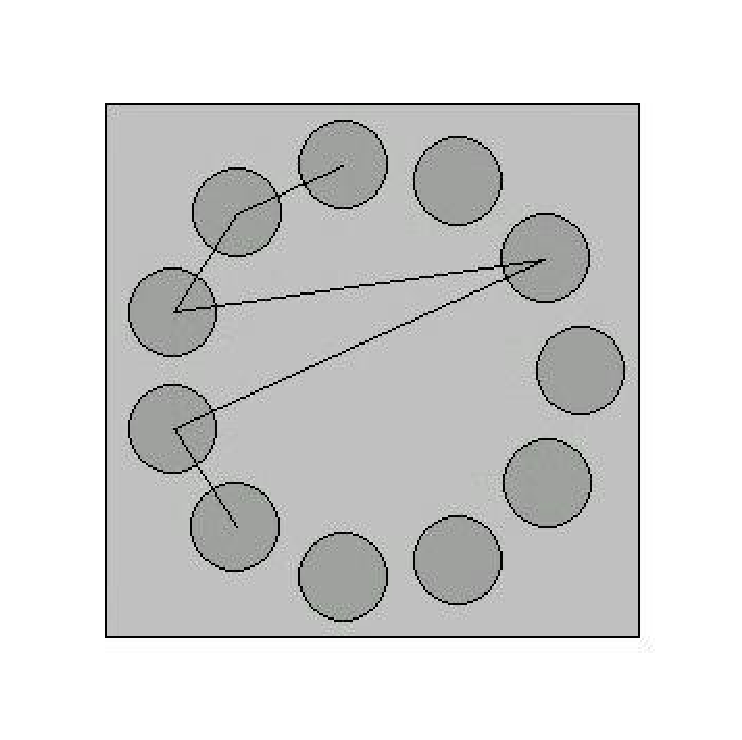
\includegraphics[angle=0,scale=0.3]{heatavi3.eps} \\
\end{tabular}
\caption{These three figures, from left to right, were captured from OverView when an actor was created. 
The outer square represents a SALSA theater, while the inner circles 
represent SALSA actors. Lines between actors represent SALSA message sending behavior.}
\label{heatExample}
\end{figure}

\emph{Please note that OverView requires Java 1.5 to compile and run.}

\section{Using OverView with SALSA Programs}
To visualize SALSA programs, we instrument SALSA (that is, insert event-sending behavior) into SALSA itself; in this way, any executed SALSA program may be visualized, if desired, without any additional configuration.

The easiest way to use OverView to visualize SALSA programs is to download the latest OverView-instrumented SALSA binary, which can be found at:
\begin{description}
  \item {\tt http://wcl.cs.rpi.edu/overview/}
\end{description}

You should download {\tt overview<version>.jar} and {\tt salsa<version>i.jar}, and place them in a convenient location. When executing your SALSA application, simply ensure that both JAR files are in your Java classpath (by either using the {/tt CLASSPATH} environment variable, or by using the {\tt -cp} command line switch).

\emph{If you wish to compile OverView and SALSA from source and instrument SALSA yourself, please see the respective documentations for OverView and SALSA.}

To run OverView and visualize your SALSA application, you must keep in mind that {\tt event sinks} must be started before {\tt event sources}; in practical terms, this means that the OverView visualization must be running before you start your SALSA program.

To do so is relatively simple: you will need an {\it OverView Daemon} (OVD) to collect and forward events, and an {\it OverView Presenter} (OVP) to display the visualization.

\begin{description}
  \item{\tt java overview.ovd.OverViewDaemon}
  \item{\tt java overview.ovp.OverViewPresenter <host:port of OVD>}
\end{description}

\emph{If you are running OVP and OVD on the same machine, OVD's host:port will generally be {\tt localhost:6060}.}

After OverView is running, you may start your SALSA theaters, name servers, and so on. Merely note that every SALSA program that is run (including theaters!) must have the command line switch {\tt -DovHost=<host:port of OVD>} to enable event sending, and to tell SALSA where to send events.

\emph{If you wish to use the instrumented version of SALSA without OverView, simply don't specify {\tt -DovHost}! SALSA programs will then run as usual, without trying to send events.}
 
You can test OverView and SALSA with the following SALSA example:
{\sloppy
\begin{description}
  \item{\tt java -DovHost=<host:port of OVD> examples.fibonacci.Fibonacci 6}
\end{description}
}

You should begin to see a visualization of the sequence of Fibonacci numbers being calculated recursively, using SALSA actors.

\chapter{History of SALSA}
SALSA has been developed since 1998 by Carlos A. Varela, who was a Ph.D. student directed by Gul Agha at
University of Illinois at Urbana-Champaign (UIUC). During the UIUC period, Gregory Haik, a student of Gul Agha, 
has contributions to the naming service of the very early SALSA. 
Carlos A. Varela founded the Worldwide Computing Laboratory and continued the development of SALSA
when he became a faculty member at Rensselaer Polytechnic Institute in 2001.
Many of his students have participated in the SALSA project since then,
including Wei-Jen Wang,
Travis Desell, Kaoutar El Maghraoui, Jason LaPorte,
Abe Stephens, and Robin Toll.
Abe Stephens and Travis Desell were the major contributors of the early version of SALSA at RPI.
They worked together from 2001 until Abe Stephens graduated. Robin Toll has helped 
the early SALSA compiler during this period of time.
From 2003 to 2004, Travis Desell has committed a thoroughly change on the early SALSA, which then became the
foundation of the current version of SALSA. Advanced features such as message properties, 
name tokens, and join block continuations were introduced at that time. 
Wei-Jen Wang and Kaoutar El Maghraoui joined the SALSA project since 2003.
Kaoutar El Maghraoui has major contributions to the development of the communication layer of 
the latest SALSA.
Wei-Jen Wang has been a major developer since 2004. 
He made another major change on SALSA in 2004 and released it in 2005. 
He introduced actor garbage collection,
fault-tolerance communication using persistent sockets and messages, 
actor name deletion support for naming services, and passing-by-value message delivery.      
Jason LaPorte joined the SALSA project in 2006. His contributions relate to  
the interface between SALSA and the OverView project.   

\chapter{SALSA Grammar}\label{GRAMMAR}{
The SALSA grammar is listed as follows:
%begin{latexonly} 
{\singlespace
\lstinputlisting[frame=no]{code/grammar.txt}
}
%end{latexonly} 
\begin{htmlonly}
 \begin{rawhtml} 
  <table border="1" cellpadding="2" cellspacing="0" style="border-collapse: collapse" bordercolor="#111111" id="AutoNumber1">
   <tr><td><pre>
  \end{rawhtml} 
\input{htmlcode/grammar.txt}
 \begin{rawhtml} 
   </pre></td></tr>
  </table>
\end{rawhtml} 
\end{htmlonly}

}
